\setcounter{definition}{0} \setcounter{property}{0} \setcounter{claim}{0} \setcounter{fact}{0} \setcounter{corollary}{0} \setcounter{figure}{0}
\section{Shortest Path Tree}

So far we have designed three algorithms, BFS, Dijkstra's algorithm, and Bellman-Ford algorithm
to solve shortest path problems for unit edge length, positive edge length, and possible negative edge length.
In these algorithm, $dist[v]$ will give the \emph{length} of the
shortest path from $s$ to $v$. How to find the actual shortest path?
Before designing algorithm to find paths~(we will do it by modifying all three algorithm),
let's think about how to store them first.
Recall that we want to store $|V|$ paths, ones from $s$ to each vertex in $V$.
If we explicitly store these $|V|$ paths in a naive way, it may take $O(|V|^2)$ space.
Can we do better?

In fact, we can use linear space to store these $|V|$ shortest paths from a single source $s$.
How is that possible? The reason is the \emph{optimal substructure} property that the shortest path problem satisfies.
Assume $s = v_0 \to v_1 \to v_2\cdots v_k$ be the shortest path from $s$ to $v_k$. Then $s \to v_i$, for any $0 \le i < k$,
is also the one shortest path from $s$ to $v_i$. This implies that storing the path from $s$ to $v_k$ is enough to
represent the shortest paths from $s$ to each $v_i$. 

But one such path is not enough to represent all shortest paths from $s$. In fact, all shortest paths
can be represented as a tree, called \emph{shortest path tree}.
%Let $G = (V, E)$ be a graph with edge length $l(e)$ for any $e \in E$.
%Here we allow negative edge length, but not allow \emph{negative cycle}. %~(we will come back to negative cycle later on).
%Let $s \in V$ be a source vertex in graph $G = (V, E)$.  
Without loss of generality, assume that source $s$ can reach all vertices in $V$.
We say $T$ is a \emph{shortest path tree} of $G$ w.r.t.\ source vertex $s$ if:
\vspace*{-\topsep}
\begin{enumerate}
\item $T$ is a rooted tree and its root is $s$;
\item vertices of $T$ is $V$;
\item edges of $T$ is a subset of $E$;
\item for every $v\in V$, the unique path from $s$ to $v$ in $T$ is one shortest path from $s$ to $v$ in $G$.
\end{enumerate}

We will show later that, a shortest path tree always exists. %(Think how to prove it.) 
%The underlying reason is the optimal substructure property.
Such tree may not be unique though~(see Figure~\ref{fig:tree}).
As in the shortest path tree, each vertex, except $s$, has exactly one in-edge, we can use an array $prev$ of size $|V|$
to store this tree. Array $prev$ is indexed by the vertices, and for each $v\in V$, $prev[v]$ stores the parent of $v$
in the tree~(see Figure~\ref{fig:tree}).
Such array, which takes linear space, therefore represents the shortest path from $s$ to every vertex.

\begin{figure}[h]
\centering{

\tikzset{every picture/.style={line width=0.75pt}} %set default line width to 0.75pt        

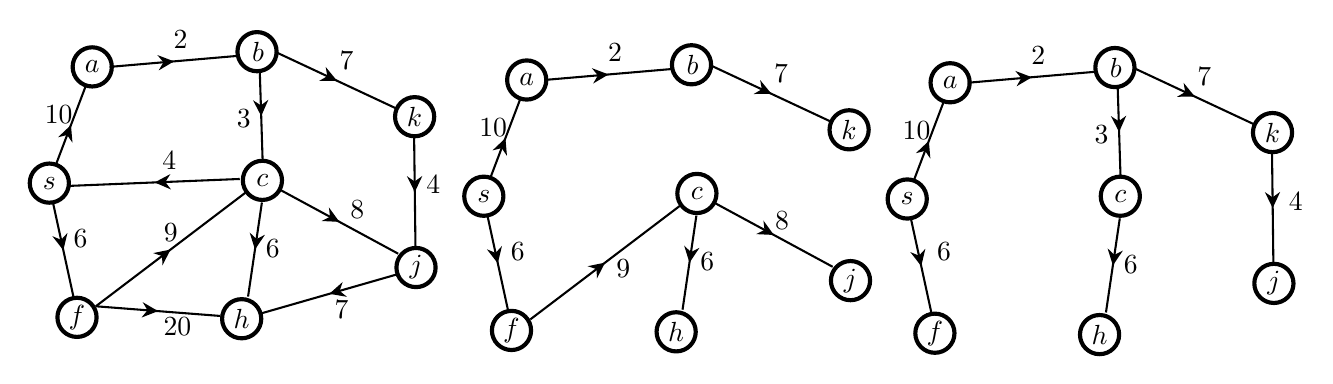
\begin{tikzpicture}[x=0.5pt,y=0.5pt,yscale=-1,xscale=1]
%uncomment if require: \path (0,296); %set diagram left start at 0, and has height of 296

%Straight Lines [id:da13938130506478386] 
\draw [color={rgb, 255:red, 0; green, 0; blue, 0 }  ,draw opacity=1 ][line width=0.75]    (71,46) -- (164,38) ;
\draw [shift={(117.5,42)}, rotate = 535.0799999999999] [fill={rgb, 255:red, 0; green, 0; blue, 0 }  ,fill opacity=1 ][line width=0.08]  [draw opacity=0] (11.61,-5.58) -- (0,0) -- (11.61,5.58) -- (7.71,0) -- cycle    ;
%Straight Lines [id:da9726442109555397] 
\draw [color={rgb, 255:red, 0; green, 0; blue, 0 }  ,draw opacity=1 ][line width=0.75]    (42,132) -- (165,127) ;
\draw [shift={(103.5,129.5)}, rotate = 357.67] [fill={rgb, 255:red, 0; green, 0; blue, 0 }  ,fill opacity=1 ][line width=0.08]  [draw opacity=0] (11.61,-5.58) -- (0,0) -- (11.61,5.58) -- (7.71,0) -- cycle    ;
%Straight Lines [id:da448389007016626] 
\draw [color={rgb, 255:red, 0; green, 0; blue, 0 }  ,draw opacity=1 ][line width=0.75]    (61,219) -- (169,137) ;
\draw [shift={(115,178)}, rotate = 502.79] [fill={rgb, 255:red, 0; green, 0; blue, 0 }  ,fill opacity=1 ][line width=0.08]  [draw opacity=0] (11.61,-5.58) -- (0,0) -- (11.61,5.58) -- (7.71,0) -- cycle    ;
%Straight Lines [id:da5032683124951551] 
\draw [color={rgb, 255:red, 0; green, 0; blue, 0 }  ,draw opacity=1 ][line width=0.75]    (61,219) -- (151,226) ;
\draw [shift={(106,222.5)}, rotate = 184.45] [fill={rgb, 255:red, 0; green, 0; blue, 0 }  ,fill opacity=1 ][line width=0.08]  [draw opacity=0] (11.61,-5.58) -- (0,0) -- (11.61,5.58) -- (7.71,0) -- cycle    ;
%Straight Lines [id:da4693132389867697] 
\draw [color={rgb, 255:red, 0; green, 0; blue, 0 }  ,draw opacity=1 ][line width=0.75]    (278,76) -- (192.5,36) ;
\draw [shift={(235.25,56)}, rotate = 205.07] [fill={rgb, 255:red, 0; green, 0; blue, 0 }  ,fill opacity=1 ][line width=0.08]  [draw opacity=0] (11.61,-5.58) -- (0,0) -- (11.61,5.58) -- (7.71,0) -- cycle    ;
%Straight Lines [id:da11523655111432152] 
\draw [color={rgb, 255:red, 0; green, 0; blue, 0 }  ,draw opacity=1 ][line width=0.75]    (291,96) -- (292,177) ;
\draw [shift={(291.5,136.5)}, rotate = 269.29] [fill={rgb, 255:red, 0; green, 0; blue, 0 }  ,fill opacity=1 ][line width=0.08]  [draw opacity=0] (11.61,-5.58) -- (0,0) -- (11.61,5.58) -- (7.71,0) -- cycle    ;
%Straight Lines [id:da5670968769979783] 
\draw [color={rgb, 255:red, 0; green, 0; blue, 0 }  ,draw opacity=1 ][line width=0.75]    (279.5,181) -- (194.5,135) ;
\draw [shift={(237,158)}, rotate = 208.42] [fill={rgb, 255:red, 0; green, 0; blue, 0 }  ,fill opacity=1 ][line width=0.08]  [draw opacity=0] (11.61,-5.58) -- (0,0) -- (11.61,5.58) -- (7.71,0) -- cycle    ;
%Straight Lines [id:da19990166326716485] 
\draw [color={rgb, 255:red, 0; green, 0; blue, 0 }  ,draw opacity=1 ][line width=0.75]    (171,212) -- (181,144) ;
\draw [shift={(176,178)}, rotate = 278.37] [fill={rgb, 255:red, 0; green, 0; blue, 0 }  ,fill opacity=1 ][line width=0.08]  [draw opacity=0] (11.61,-5.58) -- (0,0) -- (11.61,5.58) -- (7.71,0) -- cycle    ;
%Straight Lines [id:da4620737362473012] 
\draw [color={rgb, 255:red, 0; green, 0; blue, 0 }  ,draw opacity=1 ][line width=0.75]    (181,224) -- (278.5,196) ;
\draw [shift={(229.75,210)}, rotate = 343.98] [fill={rgb, 255:red, 0; green, 0; blue, 0 }  ,fill opacity=1 ][line width=0.08]  [draw opacity=0] (11.61,-5.58) -- (0,0) -- (11.61,5.58) -- (7.71,0) -- cycle    ;
%Straight Lines [id:da5742144835686415] 
\draw [color={rgb, 255:red, 0; green, 0; blue, 0 }  ,draw opacity=1 ][line width=0.75]    (181.5,113) -- (179.5,50) ;
\draw [shift={(180.5,81.5)}, rotate = 268.18] [fill={rgb, 255:red, 0; green, 0; blue, 0 }  ,fill opacity=1 ][line width=0.08]  [draw opacity=0] (11.61,-5.58) -- (0,0) -- (11.61,5.58) -- (7.71,0) -- cycle    ;
%Straight Lines [id:da5224473384909644] 
\draw [color={rgb, 255:red, 0; green, 0; blue, 0 }  ,draw opacity=1 ][line width=0.75]    (54,59) -- (32,117) ;
\draw [shift={(43,88)}, rotate = 110.77] [fill={rgb, 255:red, 0; green, 0; blue, 0 }  ,fill opacity=1 ][line width=0.08]  [draw opacity=0] (11.61,-5.58) -- (0,0) -- (11.61,5.58) -- (7.71,0) -- cycle    ;
%Straight Lines [id:da06829368652991663] 
\draw [color={rgb, 255:red, 0; green, 0; blue, 0 }  ,draw opacity=1 ][line width=0.75]    (30,144) -- (45,213) ;
\draw [shift={(37.5,178.5)}, rotate = 257.74] [fill={rgb, 255:red, 0; green, 0; blue, 0 }  ,fill opacity=1 ][line width=0.08]  [draw opacity=0] (11.61,-5.58) -- (0,0) -- (11.61,5.58) -- (7.71,0) -- cycle    ;
%Straight Lines [id:da324051151082301] 
\draw [color={rgb, 255:red, 0; green, 0; blue, 0 }  ,draw opacity=1 ][line width=0.75]    (385,55.47) -- (478,47.47) ;
\draw [shift={(431.5,51.47)}, rotate = 535.0799999999999] [fill={rgb, 255:red, 0; green, 0; blue, 0 }  ,fill opacity=1 ][line width=0.08]  [draw opacity=0] (11.61,-5.58) -- (0,0) -- (11.61,5.58) -- (7.71,0) -- cycle    ;
%Straight Lines [id:da6457054020758902] 
\draw [color={rgb, 255:red, 0; green, 0; blue, 0 }  ,draw opacity=1 ][line width=0.75]    (375,228.47) -- (483,146.47) ;
\draw [shift={(429,187.47)}, rotate = 502.79] [fill={rgb, 255:red, 0; green, 0; blue, 0 }  ,fill opacity=1 ][line width=0.08]  [draw opacity=0] (11.61,-5.58) -- (0,0) -- (11.61,5.58) -- (7.71,0) -- cycle    ;
%Straight Lines [id:da08898044790244064] 
\draw [color={rgb, 255:red, 0; green, 0; blue, 0 }  ,draw opacity=1 ][line width=0.75]    (592,85.47) -- (506.5,45.47) ;
\draw [shift={(549.25,65.47)}, rotate = 205.07] [fill={rgb, 255:red, 0; green, 0; blue, 0 }  ,fill opacity=1 ][line width=0.08]  [draw opacity=0] (11.61,-5.58) -- (0,0) -- (11.61,5.58) -- (7.71,0) -- cycle    ;
%Straight Lines [id:da8173369145698849] 
\draw [color={rgb, 255:red, 0; green, 0; blue, 0 }  ,draw opacity=1 ][line width=0.75]    (593.5,190.47) -- (508.5,144.47) ;
\draw [shift={(551,167.47)}, rotate = 208.42] [fill={rgb, 255:red, 0; green, 0; blue, 0 }  ,fill opacity=1 ][line width=0.08]  [draw opacity=0] (11.61,-5.58) -- (0,0) -- (11.61,5.58) -- (7.71,0) -- cycle    ;
%Straight Lines [id:da05255154387758687] 
\draw [color={rgb, 255:red, 0; green, 0; blue, 0 }  ,draw opacity=1 ][line width=0.75]    (485,221.47) -- (495,153.47) ;
\draw [shift={(490,187.47)}, rotate = 278.37] [fill={rgb, 255:red, 0; green, 0; blue, 0 }  ,fill opacity=1 ][line width=0.08]  [draw opacity=0] (11.61,-5.58) -- (0,0) -- (11.61,5.58) -- (7.71,0) -- cycle    ;
%Straight Lines [id:da23878744417186581] 
\draw [color={rgb, 255:red, 0; green, 0; blue, 0 }  ,draw opacity=1 ][line width=0.75]    (368,68.47) -- (346,126.47) ;
\draw [shift={(357,97.47)}, rotate = 110.77] [fill={rgb, 255:red, 0; green, 0; blue, 0 }  ,fill opacity=1 ][line width=0.08]  [draw opacity=0] (11.61,-5.58) -- (0,0) -- (11.61,5.58) -- (7.71,0) -- cycle    ;
%Straight Lines [id:da0826949355427612] 
\draw [color={rgb, 255:red, 0; green, 0; blue, 0 }  ,draw opacity=1 ][line width=0.75]    (344,153.47) -- (359,222.47) ;
\draw [shift={(351.5,187.97)}, rotate = 257.74] [fill={rgb, 255:red, 0; green, 0; blue, 0 }  ,fill opacity=1 ][line width=0.08]  [draw opacity=0] (11.61,-5.58) -- (0,0) -- (11.61,5.58) -- (7.71,0) -- cycle    ;
%Straight Lines [id:da07055049986463535] 
\draw [color={rgb, 255:red, 0; green, 0; blue, 0 }  ,draw opacity=1 ][line width=0.75]    (691,57.47) -- (784,49.47) ;
\draw [shift={(737.5,53.47)}, rotate = 535.0799999999999] [fill={rgb, 255:red, 0; green, 0; blue, 0 }  ,fill opacity=1 ][line width=0.08]  [draw opacity=0] (11.61,-5.58) -- (0,0) -- (11.61,5.58) -- (7.71,0) -- cycle    ;
%Straight Lines [id:da3797107008310523] 
\draw [color={rgb, 255:red, 0; green, 0; blue, 0 }  ,draw opacity=1 ][line width=0.75]    (898,87.47) -- (812.5,47.47) ;
\draw [shift={(855.25,67.47)}, rotate = 205.07] [fill={rgb, 255:red, 0; green, 0; blue, 0 }  ,fill opacity=1 ][line width=0.08]  [draw opacity=0] (11.61,-5.58) -- (0,0) -- (11.61,5.58) -- (7.71,0) -- cycle    ;
%Straight Lines [id:da3245212823908151] 
\draw [color={rgb, 255:red, 0; green, 0; blue, 0 }  ,draw opacity=1 ][line width=0.75]    (911,107.47) -- (912,188.47) ;
\draw [shift={(911.5,147.97)}, rotate = 269.29] [fill={rgb, 255:red, 0; green, 0; blue, 0 }  ,fill opacity=1 ][line width=0.08]  [draw opacity=0] (11.61,-5.58) -- (0,0) -- (11.61,5.58) -- (7.71,0) -- cycle    ;
%Straight Lines [id:da7475434016298388] 
\draw [color={rgb, 255:red, 0; green, 0; blue, 0 }  ,draw opacity=1 ][line width=0.75]    (791,223.47) -- (801,155.47) ;
\draw [shift={(796,189.47)}, rotate = 278.37] [fill={rgb, 255:red, 0; green, 0; blue, 0 }  ,fill opacity=1 ][line width=0.08]  [draw opacity=0] (11.61,-5.58) -- (0,0) -- (11.61,5.58) -- (7.71,0) -- cycle    ;
%Straight Lines [id:da2662386303257822] 
\draw [color={rgb, 255:red, 0; green, 0; blue, 0 }  ,draw opacity=1 ][line width=0.75]    (801.5,124.47) -- (799.5,61.47) ;
\draw [shift={(800.5,92.97)}, rotate = 268.18] [fill={rgb, 255:red, 0; green, 0; blue, 0 }  ,fill opacity=1 ][line width=0.08]  [draw opacity=0] (11.61,-5.58) -- (0,0) -- (11.61,5.58) -- (7.71,0) -- cycle    ;
%Straight Lines [id:da4243001122914827] 
\draw [color={rgb, 255:red, 0; green, 0; blue, 0 }  ,draw opacity=1 ][line width=0.75]    (674,70.47) -- (652,128.47) ;
\draw [shift={(663,99.47)}, rotate = 110.77] [fill={rgb, 255:red, 0; green, 0; blue, 0 }  ,fill opacity=1 ][line width=0.08]  [draw opacity=0] (11.61,-5.58) -- (0,0) -- (11.61,5.58) -- (7.71,0) -- cycle    ;
%Straight Lines [id:da6676082423911365] 
\draw [color={rgb, 255:red, 0; green, 0; blue, 0 }  ,draw opacity=1 ][line width=0.75]    (650,155.47) -- (665,224.47) ;
\draw [shift={(657.5,189.97)}, rotate = 257.74] [fill={rgb, 255:red, 0; green, 0; blue, 0 }  ,fill opacity=1 ][line width=0.08]  [draw opacity=0] (11.61,-5.58) -- (0,0) -- (11.61,5.58) -- (7.71,0) -- cycle    ;

% Text Node
\draw (115.24,18.06) node [anchor=north west][inner sep=0.75pt]   [align=left] {$\displaystyle 2$};
% Text Node
\draw  [line width=1.5]   (27.38, 130) circle [x radius= 14.15, y radius= 14.15]   ;
\draw (27.38,130) node   [align=left] {$\displaystyle s$};
% Text Node
\draw  [line width=1.5]   (58.38, 46) circle [x radius= 14.15, y radius= 14.15]   ;
\draw (58.38,46) node   [align=left] {$\displaystyle a$};
% Text Node
\draw  [line width=1.5]   (177.48, 35) circle [x radius= 14.15, y radius= 14.15]   ;
\draw (171.98,35) node [anchor=west] [inner sep=0.75pt]   [align=left] {$\displaystyle b$};
% Text Node
\draw  [line width=1.5]   (181.38, 128) circle [x radius= 14.15, y radius= 14.15]   ;
\draw (181.38,128) node   [align=left] {$\displaystyle c$};
% Text Node
\draw  [line width=1.5]   (291.38, 82) circle [x radius= 14.15, y radius= 14.15]   ;
\draw (291.38,82) node   [align=left] {$\displaystyle k$};
% Text Node
\draw  [line width=1.5]   (166.38, 228) circle [x radius= 14.15, y radius= 14.15]   ;
\draw (166.38,228) node   [align=left] {$\displaystyle h$};
% Text Node
\draw  [line width=1.5]   (47.38, 227) circle [x radius= 14.15, y radius= 14.15]   ;
\draw (47.38,227) node   [align=left] {$\displaystyle f$};
% Text Node
\draw  [line width=1.5]   (292.38, 191) circle [x radius= 14.15, y radius= 14.15]   ;
\draw (292.38,191) node   [align=left] {$\displaystyle j$};
% Text Node
\draw (22.24,72.06) node [anchor=north west][inner sep=0.75pt]   [align=left] {$\displaystyle 10$};
% Text Node
\draw (107.24,105.06) node [anchor=north west][inner sep=0.75pt]   [align=left] {$\displaystyle 4$};
% Text Node
\draw (108.24,157.06) node [anchor=north west][inner sep=0.75pt]   [align=left] {$\displaystyle 9$};
% Text Node
\draw (108,225.5) node [anchor=north west][inner sep=0.75pt]   [align=left] {$\displaystyle 20$};
% Text Node
\draw (235.24,33.06) node [anchor=north west][inner sep=0.75pt]   [align=left] {$\displaystyle 7$};
% Text Node
\draw (243,141) node [anchor=north west][inner sep=0.75pt]   [align=left] {$\displaystyle 8$};
% Text Node
\draw (231.75,213) node [anchor=north west][inner sep=0.75pt]   [align=left] {$\displaystyle 7$};
% Text Node
\draw (298,122.47) node [anchor=north west][inner sep=0.75pt]   [align=left] {$\displaystyle 4$};
% Text Node
\draw (161,75) node [anchor=north west][inner sep=0.75pt]   [align=left] {$\displaystyle 3$};
% Text Node
\draw (182,169) node [anchor=north west][inner sep=0.75pt]   [align=left] {$\displaystyle 6$};
% Text Node
\draw (429.24,27.53) node [anchor=north west][inner sep=0.75pt]   [align=left] {$\displaystyle 2$};
% Text Node
\draw  [line width=1.5]   (341.38, 139.47) circle [x radius= 14.15, y radius= 14.15]   ;
\draw (341.38,139.47) node   [align=left] {$\displaystyle s$};
% Text Node
\draw  [line width=1.5]   (372.38, 55.47) circle [x radius= 14.15, y radius= 14.15]   ;
\draw (372.38,55.47) node   [align=left] {$\displaystyle a$};
% Text Node
\draw  [line width=1.5]   (491.48, 44.47) circle [x radius= 14.15, y radius= 14.15]   ;
\draw (485.98,44.47) node [anchor=west] [inner sep=0.75pt]   [align=left] {$\displaystyle b$};
% Text Node
\draw  [line width=1.5]   (495.38, 137.47) circle [x radius= 14.15, y radius= 14.15]   ;
\draw (495.38,137.47) node   [align=left] {$\displaystyle c$};
% Text Node
\draw  [line width=1.5]   (605.38, 91.47) circle [x radius= 14.15, y radius= 14.15]   ;
\draw (605.38,91.47) node   [align=left] {$\displaystyle k$};
% Text Node
\draw  [line width=1.5]   (480.38, 237.47) circle [x radius= 14.15, y radius= 14.15]   ;
\draw (480.38,237.47) node   [align=left] {$\displaystyle h$};
% Text Node
\draw  [line width=1.5]   (361.38, 236.47) circle [x radius= 14.15, y radius= 14.15]   ;
\draw (361.38,236.47) node   [align=left] {$\displaystyle f$};
% Text Node
\draw  [line width=1.5]   (606.38, 200.47) circle [x radius= 14.15, y radius= 14.15]   ;
\draw (606.38,200.47) node   [align=left] {$\displaystyle j$};
% Text Node
\draw (336.24,81.53) node [anchor=north west][inner sep=0.75pt]   [align=left] {$\displaystyle 10$};
% Text Node
\draw (435.24,183.53) node [anchor=north west][inner sep=0.75pt]   [align=left] {$\displaystyle 9$};
% Text Node
\draw (549.24,42.53) node [anchor=north west][inner sep=0.75pt]   [align=left] {$\displaystyle 7$};
% Text Node
\draw (550,148.47) node [anchor=north west][inner sep=0.75pt]   [align=left] {$\displaystyle 8$};
% Text Node
\draw (496,178.47) node [anchor=north west][inner sep=0.75pt]   [align=left] {$\displaystyle 6$};
% Text Node
\draw (735.24,29.53) node [anchor=north west][inner sep=0.75pt]   [align=left] {$\displaystyle 2$};
% Text Node
\draw  [line width=1.5]   (647.38, 141.47) circle [x radius= 14.15, y radius= 14.15]   ;
\draw (647.38,141.47) node   [align=left] {$\displaystyle s$};
% Text Node
\draw  [line width=1.5]   (678.38, 57.47) circle [x radius= 14.15, y radius= 14.15]   ;
\draw (678.38,57.47) node   [align=left] {$\displaystyle a$};
% Text Node
\draw  [line width=1.5]   (797.48, 46.47) circle [x radius= 14.15, y radius= 14.15]   ;
\draw (791.98,46.47) node [anchor=west] [inner sep=0.75pt]   [align=left] {$\displaystyle b$};
% Text Node
\draw  [line width=1.5]   (801.38, 139.47) circle [x radius= 14.15, y radius= 14.15]   ;
\draw (801.38,139.47) node   [align=left] {$\displaystyle c$};
% Text Node
\draw  [line width=1.5]   (911.38, 93.47) circle [x radius= 14.15, y radius= 14.15]   ;
\draw (911.38,93.47) node   [align=left] {$\displaystyle k$};
% Text Node
\draw  [line width=1.5]   (786.38, 239.47) circle [x radius= 14.15, y radius= 14.15]   ;
\draw (786.38,239.47) node   [align=left] {$\displaystyle h$};
% Text Node
\draw  [line width=1.5]   (667.38, 238.47) circle [x radius= 14.15, y radius= 14.15]   ;
\draw (667.38,238.47) node   [align=left] {$\displaystyle f$};
% Text Node
\draw  [line width=1.5]   (912.38, 202.47) circle [x radius= 14.15, y radius= 14.15]   ;
\draw (912.38,202.47) node   [align=left] {$\displaystyle j$};
% Text Node
\draw (642.24,83.53) node [anchor=north west][inner sep=0.75pt]   [align=left] {$\displaystyle 10$};
% Text Node
\draw (855.24,44.53) node [anchor=north west][inner sep=0.75pt]   [align=left] {$\displaystyle 7$};
% Text Node
\draw (781,86.47) node [anchor=north west][inner sep=0.75pt]   [align=left] {$\displaystyle 3$};
% Text Node
\draw (802,180.47) node [anchor=north west][inner sep=0.75pt]   [align=left] {$\displaystyle 6$};
% Text Node
\draw (921.24,135.06) node [anchor=north west][inner sep=0.75pt]   [align=left] {$\displaystyle 4$};
% Text Node
\draw (359,171.47) node [anchor=north west][inner sep=0.75pt]   [align=left] {$\displaystyle 6$};
% Text Node
\draw (667,171.47) node [anchor=north west][inner sep=0.75pt]   [align=left] {$\displaystyle 6$};
% Text Node
\draw (43,161.47) node [anchor=north west][inner sep=0.75pt]   [align=left] {$\displaystyle 6$};


\end{tikzpicture}

}
\caption{A directed graph and its two shortest path trees. The array representation
for the first tree is $prev[s,a,b,c,f,h,j,k] = [null, s, a, f, s, c, c, b]$.}
\label{fig:tree}
\end{figure}


%\subsection*{Determining Shortest Path Tree}

We now modify the three algorithms, BFS, Dijkstra's algorithm, and Bellman-Ford algorithm, to allow them to generate a shortest path tree.
The idea is that, %to keep track of its predecessor of each vertex~(essentially the parent of $v$ in the shortest path tree).
%We use array $prev$ of size $|V|$ to do it.
whenever $dist[v]$ gets updated as $dist[u] + l(u,v)$ we also immediately assign $prev[v]$ as $u$.
See their pseudo-codes below.

\begin{minipage}{0.8\textwidth}
	\aaA {17}{Algorithm BFS~($G = (V, E), s \in V$)}\xxx
	\aab {$dist[v] = \infty$, for any $v\in V$;}\xxx
	\aab {\textcolor{blue}{$prev[v] = null$, for any $v\in V$};}\xxx
	\aab {init an empty queue $Q$;}\xxx
	\aab {$dist[s] = 0$;}\xxx
	\aab {insert~($Q, s$);}\xxx
	\aaB {9}{while~(empty~($Q$) = false)}\xxx
	\aac {$u$ = find-earliest~($Q$);}\xxx
	\aac {delete-earliest~($Q$);}\xxx
	\aaC {5}{for each edge~$(u, v)\in E$}\xxx
	\aaD {4}{if~($dist[v] = \infty$)}\xxx
	\aae {$dist[v] = dist[u] + 1$;}\xxx
	\aae {\textcolor{blue}{$prev[v] = u$;}}\xxx
	\aae {insert~($Q$, $v$);}\xxx
	\aad {end if;}\xxx
	\aac {end for;}\xxx
	\aab {end while;}\xxx
	\aaa {end algorithm;}\xxx
\end{minipage}


\begin{minipage}{0.8\textwidth}
	\aaA {18}{Algorithm Dijkstra~($G = (V, E)$, $l(e)$ for any $e\in E$, $s \in V$)}\xxx
	\aab {$dist[v] = \infty$, for any $v\in V$;}\xxx
	\aab {\textcolor{blue}{$prev[v] = null$, for any $v\in V$};}\xxx
	\aab {init an empty priority queue $PQ$;}\xxx
	\aab {for any $v\in V$: insert~($PQ$, $v$), where the priority of $v$ is $\infty$;}\xxx
	\aab {$dist[s] = 0$;}\xxx
	\aab {decrease-key~($PQ, s, 0$);}\xxx
	\aaB {10}{while~(empty~($PQ$) = false)}\xxx
	\aac {$u$ = find-min~($PQ$);}\xxx
	\aac {delete-min~($PQ$);}\xxx
	\aaC {6}{for each edge~$(u, v)\in E$}\xxx
	\aaD {4}{if~($dist[v] > dist[u] + l(u,v)$)}\xxx
	\aae {$dist[v] = dist[u] + l(u,v)$;}\xxx
	\aae {\textcolor{blue}{$prev[v] = u$;}}\xxx
	\aae {decrease-key~($PQ$, $v$, $dist[v]$);}\xxx
	\aad {end if;}\xxx
	\aac {end for;}\xxx
	\aab {end while;}\xxx
	\aaa {end algorithm;}\xxx
\end{minipage}

\begin{minipage}{0.8\textwidth}
	\aaA {9}{Algorithm Bellman-Ford~($G = (V, E)$, $l(e)$ for any $e\in E$, $s \in V$)}\xxx
	\aab {init an array $dist$ of size $|V|$;}\xxx
	\aab {$dist[s] = 0$; $dist[v] = \infty$ for any $v\neq s$;}\xxx
	\aab {\textcolor{blue}{$prev[v] = null$, for any $v\in V$};}\xxx
	\aaB {4}{for $k = 1 \to |V| - 1$}\xxx
	\aaC {2}{for each edge $(u,v)\in E$}\xxx
	\aad {$update(u,v)$;}\xxx
	\aac {end for;}\xxx
	\aab {end for;}\xxx
%	\aab {report: $dist[v]$ gives $distance(s,v)$, for any $v\in V$;}\xxx
	\aaa {end algorithm;}\xxx
\end{minipage}

\begin{minipage}{0.8\textwidth}
	\aaA {5}{procedure update~(edge $(u,v)\in E$)}\xxx
	\aaB {3}{if~($dist[v] > dist[u] + l(u,v)$)}\xxx
	\aac {$dist[v] = dist[u] + l(u,v)$;}\xxx
	\aac {\textcolor{blue}{$prev[v]= u$};}\xxx
	\aab {end if;}\xxx
	\aaa {end procedure;}\xxx
\end{minipage}


The resulting $prev$ array corresponds to a graph called $T$, in which the vertices are $V$
and edges are $\{(prev[v], v)\mid v\in V\}$. We now prove that this graph is indeed one shortest path tree,
by showing $T$ satisfying the 4 conditions in the definition. It is trivial to verify that the conditions (2)
is satisfied, as the vertices are $V$; condition (3) is easy as well, as in any of the algorithm,
assigning $u$ to $prev[v]$ already happens when examining edge $(u,v)\in E$.
Below we then prove condition (1) and (4).

\begin{fact}
\label{tree-fact2}
At any time of the algorithm, for any $v\in V$, let $u = prev[v]$, if $u\neq null$ then $dist[v] = dist[u] + l(u,v)$;
in particular, when the algorithm terminates, we have $distance(s,v) = distance(s,u) + l(u,v)$.
\end{fact}
The first part of above fact is a direct consequence of each algorithm as we update $prev$ right after updating $dist[v]$ as $dist[u] + l(u,v)$.
The secon part also uses the correctness of each algorithm, i.e., when each algorithm terminates, we have $dist[v] = distance(s,v)$.

We now prove condition (1), i.e., $T$ is a tree with root being $s$~(although we use $T$ but we have not showed that it is a tree).
Since $T$ corresponds to array $prev$, it is obvious that in-degree of $s$ is 0 and that each vertex in $T$, except $s$,
has in-degree of 1. We therefore just need to prove that $T$ does not contain cycle. 
We need a stronger assumption to make it true. That is, the graph $G$ cannot contain negative nor length-zero cycles.

\begin{fact}
$T$ does not contain cycle, if all cycles in $G$ are of positive length.
\end{fact}
\emph{Proof.} Suppose conversely that there exists a cycle $C = v_1\to v_2\to \cdots \to v_k\to v_1$ in $T$.
Following above fact, we have $dist[v_i] = dist[v_{i-1}] + l(v_{i-1},v_i)$, for every $1 < i \le k$
and $dist[v_1] = dist[v_k] + l(v_k,v_1)$.
Summing up both sides gives $\sum_{e\in C} l(e) = 0$, contradicting to the the assumption
that all cycles have positive length.\qed

Last, we prove condition (4):
\begin{claim}
For every $v\in V$, the unique path from $s$ to $v$ in $T$ is one shortest path from $s$ to $v$ in $G$,
if all cycles in $G$ are positive cycles.
\end{claim}
\emph{Proof.} 
Let $p: s = v_0 \to v_1 \to v_2 \to \cdots \to v_k$ be the path from $s$ to $v_k$ in $T$.
By the construction of $T$, we know that $prev[v_i] = v_{i - 1}$, $1\le i \le k$.
Therefore, using Fact~\ref{tree-fact2}, we have $distance(s, v_i) = distance(s, v_{i-1}) + l(v_{i-1}, v)$,
for each $i = 1, 2, \cdots, k$. We sum up the left side and the right side of these $k$ equations.
Canceling out $distance(s, v_i)$, $i = 1, 2, \cdots, k-1$, on both sides gives
$distance(s,v_k) = distance(s, s) + \sum_{i=1}^k l(v_{i-1}, v_i) = \sum_{i=1}^k l(v_{i-1}, v_i)$, implying that
the length of $p$ is equal to the distance from $s$ to $v_k$, i.e., it is one shortest path from $s$ to $v_k$. \qed


